%%%%%%%%%%%%%%%%%%%%%%%%%%%%%%%%%%%%%%%%%%%%%%%%%%%%%%%%%%%%%%%%%%% 
%                                                                 %
%                            CHAPTER THREE                          %
%                                                                 %
%%%%%%%%%%%%%%%%%%%%%%%%%%%%%%%%%%%%%%%%%%%%%%%%%%%%%%%%%%%%%%%%%%% 
 

\chapter{EXTENDED BALANCE THEORY} \label{sec:esbt}
In Heider's balance theory~\cite{Heider:46}, relations are restricted to binary values
($+$/$-$). When Cartwright
and Harrary first formalized the theory of structural balance, they
also suggested that relationships of interest exist in varying
degrees, and that their theory is built on the incomplete
representation of strengths of relations~\cite{Cartwright:56}. Tie
strength is a well-studied concept in social psychology. A person may
have close friends as well as acquaintances, strong and weak ties. A strong tie may represent a deep
trust relation spanning many constructs in high risk situations, while
a weak tie may be trusted mainly for low risk situations or for
specific constructs like providing private
information~\cite{Granovetter:1973}.

To model this distinction, we consider a scenario where relationships
have varying strengths. For example, a strong positive link represents a close
friendship or family tie, and a strong negative link represents hatred. The new balance theory in this general scenario will be called extended structural balance theory, or ESBT for short.  

Balance theory deals with the influence between interpersonal relationships, and hence a triad is the smallest unit. In a complete network in which every pair of nodes has a mutual relationship, the multilateral relationship of a subset of participants can be captured as a composition of all triads involved. When a social network is incomplete, by letting the ``no link" be a type of relationship, the same argument still holds. In other words, triad not only defines the smallest unit structure of social networks, but is also able to characterize every social structure by the composition of all triads involved. As an example, the {\it balance theorem} in SBT (WSBT) has shown the power of triad in capturing the global structure of a network. No matter how the relationship is measured (binary or varying in strengths), the center of discussion of a balance theory lies in triads: a social network is balanced if every triad involved is balanced.  

We consider a type of {\bf neutral relationship} as one that is unbiased, which will be denoted as $O$. Basically, a neutral relationship is a non-negative and non-positive relationship, corresponding to no opinion and no bias. As a result, ``no link", or ``no relationship", is a type of neutral relationship. Clearly, every combination of three nodes in a social network forms a triad if neutral relationship is considered. 

Let the collection of relations with strengths be $E$. With the introduction of neutral
relations, $E$ can be partitioned into three subsets: positive
relationships $P$, negative relations $N$ and neutral relations
$O$.  An edge $(A,B)$ and a relation with associated strength $e$ will be used interchangeably. We call $e_{1}$ is more positive (less negative) than $e_{2}$ if
\begin{enumerate}
\item $e_1$ is positive and $e_{2}$ is negative;
\item $e_{1}$, $e_{2}$ are positive, and $e_{1}$ is stronger than $e_{2}$ in strength;
\item $e_{1}$, $e_{2}$ are negative, and $e_{1}$ is weaker than $e_{2}$ in strength.
\end{enumerate}
A triad is usually denoted as $(A,B,C)$.

\section{Tolerance and Two Principles}
Reviewing the arguments in Heider's balance theory~\cite{Heider:46}, one concludes that the latent stress, or tension, causes a triad to become imbalanced. For example, in triad (4) of Figure~\ref{fig:balance_strong}, it is stressful for Alice and Chris to stay antagonistic to each other with Bob as a common friend, while Bob also feels stressed by staying friends with both Alice and Chris.  As it is argued by Davis~\cite{Davis:67}, the situation in triad (3) of Figure~\ref{fig:balance_strong} is fundamentally different. In (3), there is a {\bf possibility} that two of the nodes will ally themselves against the third. In a word, the underlying stress in imbalanced triads is the driving force that propels relationship changes. The next questions is when and how such stress rises.

We further our discussion by describing stress in terms the influence of relationships on each other within a triad. In a triad, two of its relations cause influence over the third one. Such influence restricts the range of the comfortable relations the third relation may have; if the relation goes out of the range, tension occurs and participants will suffer from stress. Participants
will seek relationship changes to resolve stress. We call
such range of relations {\bf tolerance}. Using the notion of tolerance, we can interpret
network balance at a finer level.

 For each relationship between a pair $(A,C)$ of nodes, its tolerance is constrained by the triads
$(A,C)$ is part of. If consider a single triad $(A,B,C)$, $(A,C)$'s tolerance is determined by the strengths of relations $(A,B)$ and $(B,C)$. We state the following two fundamental principles regarding tolerance:
\begin{principle}[Transitivity of positive relationships.]
Let $(A,B,C)$ be a triad of interest, and $(A,B)$, $(B,C)$ be positive. If $(A,B)$ and $(B,C)$ are more positive, $(A,C)$'s tolerance will be limited to more positive relationships.
\end{principle}
In other words, the fact that B are friends with both A and C provides
the freedom for $A$ and $C$ to become friends; and there is stress on
$A$ and $C$ to get close. The stronger the relation between $(A,B)$
and $(B,C)$, the higher the chance between $(A,C)$ to be connected
(more) positively, and the resulting tolerance is restricted to be
more positive.

The stress that is based on positive relations has been frequently
defined by SBT and WSBT. Positive relations in a triad cause stress
for the remaining relations to be positive. As a result, both in SBT
and WSBT, a balanced network consists of communities that are
connected to each other with positive ties. When we consider the
strength of relations, we generalize this by saying that the more
positive two of the relations are in a tie, there is less tolerance
for non-positive relations.

Furthermore, there is a point when the strengths of the two positive relations $(A,B)$ and $(B,C)$ are
strong enough such that it will be imbalanced for $(A,C)$ to remain
unfriended, i.e. neutral. This observation is inspired by the ``strong
triadic closure" in~\cite{Granovetter:1973}. In trust literature, for example, this is
often referred as the ``transitivity of trust'' though transitivity is
also used in other contexts.
\begin{principle} [Heterophily in relationships.] 
Let $(A,B,C)$ be a triad of interest. If the difference between $(A,B)$ and $(B,C)$ is larger, $(A,C)$'s tolerance will be limited to more negative relationships.
\end{principle}
Given individuals $A$, $B$, $C$ in a network, if the relationship
between $(A,B)$ and the relation between $(B,C)$ differs to some
extent, then the tolerance is geared towards the
negative. Furthermore, the more different the strength of the
relationships are, the tolerance is geared towards more
negative relationships. 

The second type of stress is an interpretation of homophily. We note
that homophily, i.e. having common friends or enemies, may sometimes
cause stress (in $+,+,+$) but sometimes it does not (in $-,-,-$ for
WSBT). However, lack of homophily, which we call heterophily does
cause stress. For example, consider the case $+,+,-$ for $(A,B)$,
$(B,C)$ and $(A,C)$. There is stress on $(A,C)$ to be positive due to
transitivity. But, there is also stress on $(A,B)$ or $(B,C)$ to be
negative. Either way, the result will be more desirable: either all
being friends, or having two friends with a common enemy. We call the
second type of stress the principle of heterophily. The more different
the ties are, the more pressure there is
for the tie to be negative.  At a point when the difference between
$(A,B)$ and $(B,C)$ is significant enough, we argue that a positive
relationship for $(A,C)$ will cause imbalance. This is inspired by the
observation that two people who have severely conflicted relationships
with a common neighbor, e.g., one is the other's close friend's enemy,
are not likely to friend each other.

To summarize, the tolerance of each edge in a triad is determined by the other two relationships. A triad is balanced if all three relationships in it are in the range of the corresponding tolerance. The concept of tolerance and its two principles help interpret balance in terms of relations with
strengths precisely. 

\begin{definition} [Balance]
A triad $A,B,C$ is balanced if for all pairs $(A,B)$, given the
tolerance $T(A,B)$ of $(A,B)$ with respect to $(B,C),(A,C)$,
we have that $(A,B)$ is in $T(A,B)$. 

Given a network $G$ of relationships, $G$ is said to be balanced if
for all triads in the network are balanced.
\end{definition}
\section{Measuring Relationships by Total Ordering}
To give concrete interpretations of balance in the presence of relations with strengths, we need to have a measurement of
relations. While it may appear arguable whether
the relation strengths can be expressed by numerical values, it is fairly
clear that the strength of any two relations can be compared. For
positive relations such as liking, valuing or approving, two
relationships are comparable in terms of which one is stronger than
the other. Similar argument applies to two negative
relations. Finally, a positive relation and a negative relation are
comparable by their signs. Hence, relations with strengths by nature
inherit a total ordering.
 
We pick the ordering $\preceq$
such that, $e_{1} \preceq e_{2}$ denotes $e_{1}$ is equivalently or more positive than $e_{2}$.
In the simplest case where we have only positive and negative relations, we
have that $+ \preceq -$. Following the definition of ordering $\preceq$, it is clear that
for any $e_{+} \in P$, $e_{O} \in O$, $e_{-} \in N$, $e_{+} \preceq
e_{O} \preceq e_{-}$ holds. We use $\tuple{e_1}{e_2}$ to denote the
set of relations $\tuple{e_1}{e_2}$ = $\{e\:\mid\: e_1\preceq e\preceq
e2\}$. Hence, given $\tuple{e_1}{e_2}$, the lower bound $e_1$
represents the strongest possible relationship and the upper bound
represents $e_2$ represents the weakest possible relationship in this
range.
 
Consider a single triad $(A,B,C)$, the tolerance of $(A,B)$ is of the form $\tuple{e_1}{e_2}$, a set of bounded values. That is, the range of comfortable relationships of $(A,B)$ in $(A,B,C)$ is constrained by an upper bound and a lower bound. As $(A,B)$'s tolerance is constrained by all the triads $(A,B)$ is part of, it is the intersection of all individual tolerance and hence is also of the form $\tuple{e_1}{e_2}$. Moreover, the two tolerance principles can be interpreted as the following.
\begin{principle}[Transitivity of positive relationships.]
Let individuals $A$, $B$, $C$ in a network form a triad, and $(A,B)$,
$(A,B)^{'}$, $(B,C)$ be positive. Suppose $T=\tuple{e_1}{e_2}$ denotes
the tolerance of $(A,C)$ based on relations $(A,B),(B,C)$, and
$T'=\tuple{e_1'}{e_2'}$ denotes the tolerance based on
$(A,B)^{'},(B,C)$. If $(A,B)' \preceq (A,B)$ then we have that
$e_2'\preceq e_2$.
\end{principle}{\label{ref:transitivity}
That is, if the relation between $A, B$ is changed to a more positive relation $(A,B)'$, the corresponding tolerance of $(A,C)$ will have a smaller upper bound. Equivalently, $(A,C)$'s tolerance is restricted to more positive relationships.
\begin{principle} [Heterophily in relationships.] 
Let individuals $A$, $B$, $C$ in a network form a triad. Suppose
$T=\tuple{e_1}{e_2}$ denotes the tolerance of $(A,C)$ based on
relations $(A,B),(B,C)$, and $T'=\tuple{e_1'}{e_2'}$ denotes the
tolerance based on $(A,B)^{'},(B,C)$. We have that if
$(A,B)' \preceq (A,B) \preceq (B,C)$, or $ (B,C) \preceq (A,B) \preceq
(A,B)'$, then $e_1\preceq e_1'$.
\end{principle}
That is, if the difference between $(A,B)$ and $(B,C)$ becomes larger, the corresponding tolerance of $(A,C)$ will have a larger lower bound. Equivalently, $(A,C)$'s tolerance is restricted to more negative relationships.
\begin{table}[h]
\begin{center}
\caption{\label{ref:classic_balance}Tolerance rules in structural balance theory.}
 \begin{tabular}{cc|cl} 
  $(A,B)$ & $(A,C)$ & Tolerance for $(B,C)$ &  \\ \hline
  $+$ & $+$ & $\tuple{+}{O}$ & Transitivity \\
  $+$ & $-$ & $\tuple{O}{-}$ & Heterophily \\ 
  $-$ & $-$ & $\tuple{+}{-}$ & No stress \\ 
 \end{tabular}\\\vspace{4mm}
\end{center}
\end{table}

Clearly, the binary classification of relations in classic balance theory inherits a total ordering. We give the tolerance rules for Davis's WSBT in the general case of incomplete networks in Table~\ref{ref:classic_balance}~\cite{Davis:67}. Notice that the table has neutral relationships ``$O$", which is not considered in their early work. This is because in the setting of incomplete networks, triads ``$+, +, O$" and ``$+, -, O$" are considered balanced implicitly in Davis's theory; if we substitute ``$O$" with ``$+$" in triad ``$+, +, O$" and substitute ``$O$" with ``$-$" in triad ``$+, +, O$", we can get balanced triads in WSBT~\cite{kleinberg-book}. It is easy to verify tolerance rules in Table~\ref{ref:classic_balance} agrees with Principle of Transitivity and Heterophily. According to the table, triads (1), (2) and (3) from Figure~\ref{fig:balance_strong} are balanced as each relation is within the tolerance, but triad (4) is not balanced. In this aspect, our theory is a generalization of the Davis's WSBT.
\begin{table} [htbp!]
\begin{center}
\caption{\label{ref:rel_types}Five types of relations and their
  interpretations, displayed in the ordering, i.e. $s+\preceq
  w+\preceq O\preceq w- \preceq s-$.}
\begin{tabular}{p{1.6in}p{2.6in} }
Relation Type & Interpretation \\ \hline
Strongly positive (s+) & close friendship, trust  \\ 
Weakly positive (w+) & aquiantance \\
Neutral (O) & unbiased relation, no relation  \\
Weakly negative (w-) & minor disagreement, negative bias  \\
Strongly negative (s-) & hatred, distrust  
\end{tabular}\\\vspace{4mm}
\end{center}
\end{table}

For a more detailed representation of relationships, consider a set of discrete classification of relationships shown in Table~\ref{ref:rel_types}. This classification considers relation ties that have been discussed
in previous literature.  We show how to interpret balance in
a more sophisticated manner in networks with these classes. 

{\bf Strong positive ties, s+} are similar to close
friendships. There is a strong expectation of reciprocity, similarity
of tastes (homophily), common intentions and benevolence towards each
other~\cite{Tomasello:2005}. The traditional definition of SBT is
based on these types of positive relationships.

{\bf Strong negative ties, s-} are generally explained as
having negative experiences with someone which is indicative of their
negative intentions, unreliability and overall belonging to groups
that are not considered trustworthy~\cite{Fiske:2007}. 

\begin{table}[htbp!]
\begin{center}
\caption{\label{tab:weak_strong_tolerance}Tolerance rules with strong, weak and neutral relations.}
\begin{tabular}{p{2.5in}p{2.5in}}
 \begin{tabular}{p{0.5in}p{0.5in}p{1.2in}} 
$(A,B)$ & $(A,C)$ & $(B,C)$'s tolerance \\ \hline
$s+$ & $s+$ & $\tuple{s+}{w+}$ \\
$s+$ & $w+$ & $\tuple{s+}{O}$  \\
$s+$ & O & $\tuple{s+}{w-}$ \\
$s+$ & $w-$ & $\tuple{O}{s-}$ \\ 
$s+$ & $s-$ &   $\tuple{w-}{s-}$ \\
$w+$ & $w+$ & $\tuple{s+}{w-}$ \\
$w+$ & O & $\tuple{s+}{s-}$ \\ 
$w+$ & $w-$ & $\tuple{w+}{s-}$ 
\end{tabular} &
 \begin{tabular}{p{0.5in}p{0.5in}p{1.2in}} 
$(A,B)$ & $(A,C)$ & $(B,C)$'s tolerance \\ \hline
$w+$ & $s-$ & $\tuple{O}{s-}$ \\ 
O & O & $\tuple{s+}{s-}$ \\ 
O & $w-$ & $\tuple{s+}{s-}$ \\ 
O & $s-$ &  $\tuple{w+}{s-}$ \\ 
$w-$ & $w-$ & $\tuple{s+}{s-}$ \\ 
$w-$ & $s-$ & $\tuple{s+}{s-}$ \\ 
$s-$ & $s-$ & $\tuple{s+}{s-}$ \\
& & 
\end{tabular}
\end{tabular} \\\vspace{4mm} 
\end{center}
\end{table}

However, these are not all the different classes of relationships that
one might consider in a network. Granovetter~\cite{Granovetter:1973} uses the term
weak tie to refer to a relationship that is an acquaintance, not a
close friend. Weak ties give access to less privileged information
than strong ties, but come from outside of one's close network. In
both cases, there is a tie between two people, but this
does not imply a continuous interaction or a strong affective
component as in trust.

We also introduce {\bf weak negative ties, w- } to
model cases in which there is a certain amount of distrust as a result
of biases stemming from social groups people belong to, or heresay that
may not be as strong as distrust~\cite{Ames:2011}. In essence, the
burden of proof of one's trustworthiness is much higher in weak distrust
than in distrust, but in both cases, positive evidence is not
evaluated in the same way as in trusting relations. These five types
of relationships are summarized in Table~\ref{ref:rel_types}.

The tolerance rules for networks with relations in Table~\ref{ref:rel_types} are given in Table~\ref{tab:weak_strong_tolerance}. The rules are proposed according to many early work regarding strong and weak ties, as well as common observations in real life. The
resulting imbalanced triads or structures are listed in Table~\ref{tab:imbalanced_extended}. Notice that the triads with
two positive relations and one negative relation are imbalanced as
they are in classic balance theory, except for the ones in which all
three relations as weak. In fact, the types of triads that consist
of weak relations and neutral relations only are not considered to be
imbalanced structures. Our argument here is that when all relations
are weak or neutral, the influence inside the triad is not significant
enough to draw tension. Also, triads of type ``$s+$ $s+$ O" and
``$s+$ $s-$ O" are considered to be imbalanced structures. The
arguments against each type of imbalanced structure is listed in
Table~\ref{tab:imbalanced_extended}.

\begin{table}[htbp!]
\begin{center}
\caption{\label{tab:imbalanced_extended}Imbalanced triadic structures
  in the presence of strong and weak ties, and arguments
  for the stress in the relation.} 
 \begin{tabular}{p{1.8in} p{0.2in} p{2.8in}}
Triad & &Argument for stress \\ \hline

$s+ s+ s-$, $s+ s+ w-$, $s+ w+ s-$, $s+ w+ s-$, $w+ w+ s-$ & &
my two friends cannot get along with each other \\
$s+ s+ O$ & & my two close friends do not friend each other \\ 
$s+ s- O$ & & my enemy's close friend does not pick a side\\ 
\end{tabular} \vspace{4mm}
\end{center}
\end{table}
\vspace*{-0.2in}

\section{Relation Distance and General Expression of Balance}\label{relation distance}
The concept of extended balance is meaningful only if the tolerance
rules can be explicitly defined, so that whether a triad and a network
is balanced or not can be determined. Whenever relations
are drawn from a finite ordered set, this is easy to do. However, as Cartwright and Harary also suggested, 
it is considerably more complex in the general case when the strengths
of relations are drawn from arbitrary numerical values~\cite{Cartwright:56}.
 
As a first step, we refine the measurement of relations with
strengths from total ordering to positive real values. In particular,
we define function $\psi: E \rightarrow R^{+}$ such that, for two
relations $e_{1}, e_{2} \in E$, $\psi(e_{1}) \leq \psi(e_{2})$ if and
only if $e_{1} \preceq e_{2}$.  Since positive values can be seen as
metric distances, we call $\psi(e)$ the relation distance of $e$.  In
other words, relations with varying strengths are represented by
distances with different lengths.  More negative strengths are
represented by larger distances and more positive strengths are
represented by smaller distances.

%% In the case of WSBT, Table 1 set up
%% such tolerance rules. In the extended case when strong/weak ties are
%% introduced, Table 3 provides the tolerance rules. For general cases
%% when relation strengths are not limited to particular types, however,
%% the tolerance rules are not defined. We address this problem by
%% expressing relation in terms of metric distance, based on which we set
%% up a uniform tolerance rule that generalizes Table 1 and 3.

%% In previous discussion, relations are measured by a complete
%% ordering. To express it as distance, we need an additional assumption
%% that the difference between any two relation strengths are well
%% defined. We introduce a function from relation to real values: $\psi:
%% E \rightarrow R^{+}$. For each relation $e \in E$, $\psi(e)$ denotes
%% its distance expression, which will be called relation distance for
%% simplicity. The ordering relation is then reduced to the numerical
%% comparing operator $<$.  In particular, $\psi(e_{1}) < \psi(e_{2})$ if
%% and only if $e_{1} \preceq e_{2}$.

We propose the following general rule of tolerance with the
concept of relation distance.

\begin{definition} \label{def:gen_tolerance}
Let $(A,B,C)$ be a triad of interest. The tolerance of $(A,C)$
is given by $[|\psi(A,B)-\psi(B,C)|, \psi(A,B)+\psi(B,C)]$. 
\end{definition}

It can be easily checked that the general tolerance rule agrees with
Principle 3 and 4 by substituting $\leq$ for $\preceq$.  Immediately, we have the following
theorem.
\begin{theorem} 
Given a triad $(A,B,C)$, if $\psi(A,B)$, $\psi(B,C)$, $\psi(A,C)$
satisfies the metric triangle inequality, then $(A,B,C)$ is balanced.
\end{theorem}

We first show that Table~\ref{ref:classic_balance} and Table~\ref{tab:weak_strong_tolerance} can be considered as special cases of the general tolerance rule, under a mapping of relation strengths to distances. For Davis' WSBT and its tolerance rules in Table~\ref{ref:classic_balance} , we consider two thresholds:
$b_{+} < b_{-}$ such that if $\psi(e)\geq b_{-}$ then the relationship
$e$ is negative. Similarly, if $\psi(e)\leq b_{+}$, then $e$ is
a positive relationship. For any value $b_{+} < \psi(e) < b_{-}$, the
relationship is considered neutral. We can see that as long as
$b_{-}>2b_{+}$, Table~\ref{ref:classic_balance} is equivalent to
Definition~\ref{def:gen_tolerance}.

\begin{figure}[th]
\centering
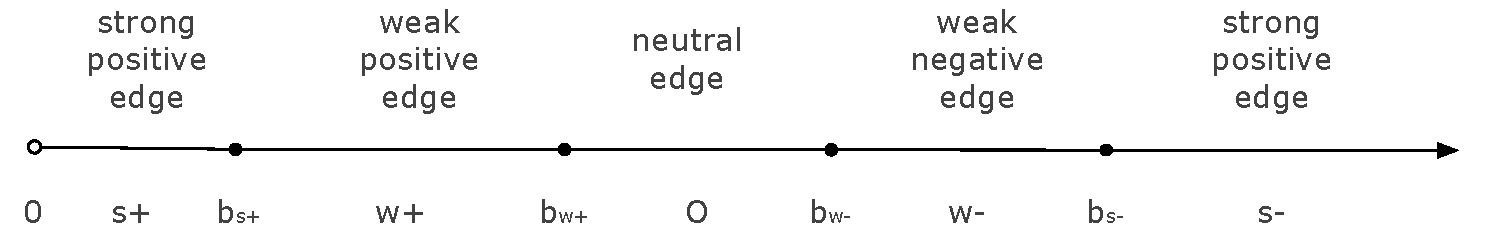
\includegraphics[height=0.7in]{Figs/mapping2.pdf}
\caption{\label{fig:partition}Partitioning of distance domain by boundary
  parameters $\{b_{s+}, b_{w+}, b_{w-}, b_{s-}\}$: distances within $(0,b_{s+}]$ are strong positive; $(b_{s+}, b_{w+})$ weak
  positive, $[b_{w+}, b_{w-}]$ neutral, $(b_{w-}, b_{s-})$
  weak negative, and $ [b_{s-}, \infty)$ strong negative.}

\end{figure}

Similarly, to capture the tolerance rules in Table~\ref{tab:weak_strong_tolerance},
we consider the partitioning of the distance domain given in
Figure~\ref{fig:partition}. We can see that if the following
conditions are satisfied for the boundary parameters: 

\begin{table}[htbp!]
\begin{center}
\caption{\label{tab:constraints}Constraints on the boundary parameters.} 
\begin{tabular}{p{2in}p{2in}}
$b_{w+}  > 2b_{s+}$ & $b_{s-}  > b_{w-} + b_{s+}$  \\
$b_{s-}  > 2b_{w+}$ & $b_{w-}  > b_{w+}+b_{s+}$
\end{tabular}{}
\end{center}
\end{table}
\vspace*{-0.2in}
then the tolerance rules given in
Table~\ref{tab:weak_strong_tolerance} are equivalent to
Definition~\ref{def:gen_tolerance}, and all triads shown in
Table~\ref{tab:imbalanced_extended} are imbalanced according to metric triangle
inequality.

With the concept of relation distance, we are able to express the
structure of a social network by drawing it in the metric
space. The strength of each relation is expressed by the distance
between two of its endpoints. Notice that evesry layout in the metric
space automatically satisfies the metric triangle inequality, and
hence corresponds to a balanced state of the network. We have the following the alternative definition of a balanced network.
\begin{definition}\label{alternative def}
Given a social network $G$, $G$ is balanced if it can be drawn in metric space such that each edge in $G$ has the length of its relation distance.
\end{definition}
%%% Local Variables: 
%%% mode: latex
%%% TeX-master: t
%%% End: 
